\documentclass[12pt]{article}

\usepackage[utf8]{inputenc}
\usepackage{color, colortbl}
\usepackage{amsmath}
\usepackage{graphicx}

\graphicspath{ {./images/} }

\mathcode`*=\string"8000
\begingroup
\catcode`*=\active
\xdef*{\noexpand\textup{\string*}}
\endgroup
\renewcommand{\baselinestretch}{1.5}
\title{Ecuaciones de DFA.}
\author{Luis Diego Jiménez Delgado\\ 2CM5}
\date{24 de septiembre del 2019}

\begin{document}
    \maketitle
    \newpage
        El automata siguiente es el que se va a desarrollar sus ecuaciones.
        \begin{center}
            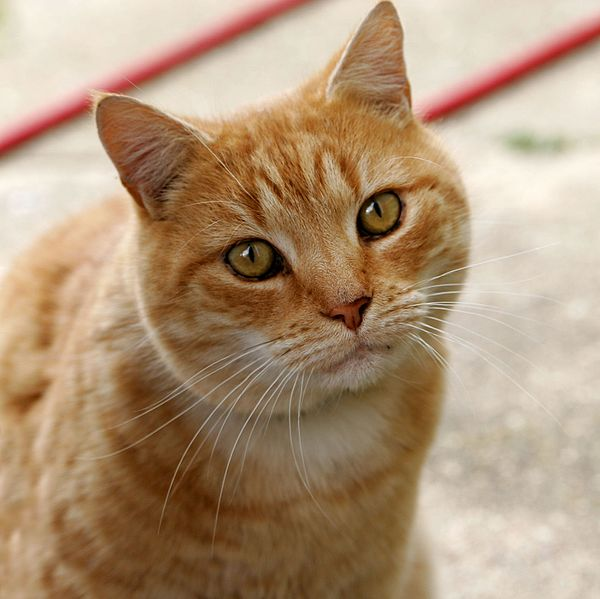
\includegraphics{a}
        \end{center}
        
\end{document}